\documentclass[12pt]{article}
\usepackage[utf8]{inputenc}
\usepackage{graphicx}
\usepackage{mathtools}
\usepackage{amsmath}
\usepackage{amsfonts}
\usepackage{amssymb}
\usepackage{amsthm}
\usepackage{enumitem}
\usepackage{centernot}
\usepackage{marvosym}
\usepackage{lscape}
\let\marvosymLightning\Lightning
\newtheorem{theorem}{Theorem}
\newtheorem{corollary}{Corollary}[theorem]
\newtheorem*{remark}{Remark}
\newtheorem{innercustomthm}{Theorem}
\newenvironment{customthm}[1]
  {\renewcommand\theinnercustomthm{#1}\innercustomthm}
  {\endinnercustomthm}
\newcommand{\subscript}[2]{$#1 _ #2$}
\newcommand{\N}{\mathbb{N}}
\newcommand{\Z}{\mathbb{Z}}
\newcommand{\R}{\mathbb{R}}
\newcommand{\C}{\mathbb{C}}
\newcommand{\F}{\mathbb{F}}
\renewcommand\qedsymbol{QED}
\newcommand{\divby}{%
  \mathrel{\text{\vbox{\baselineskip.65ex\lineskiplimit0pt\hbox{.}\hbox{.}\hbox{.}}}}%
  }
\newcommand{\notdivby}{\centernot\divby}
\newcommand\setItemnumber[1]{\setcounter{enumi}{\numexpr#1-1\relax}}
\title{\scalebox{2}{Math 431 Final Exam}}
\author{\scalebox{1.5}{Theo Koss}}
\date{December 2020}
\begin{document}
\maketitle
\section{Proof Problem (Rings):}
Let $R$ be a ring. An idempotent of $R$ is some element $a\in R$ such that $a^2=a$. E.g. 1 in a ring with unity. Suppose $R$ is a ring with unity and $a\in R$ is an idempotent element. Prove the following:
\begin{enumerate}[label=(\alph*)]
    \item $a(1-a)$ is an idempotent.
    \begin{proof}
    $a(1-a)=a-a^2$. Replacing $a$ with $a^2$ we get: $a^2(1-a^2)=a^2-a^4$. Since $a=a^2$, these are equal, $a-a^2=a^2-a^4$. There are exactly 2 $a\in R$ for which this is true, $a=0,1$. Now it is easy to check, a given element $b$ is idempotent iff $b=0$ or $b=1$. For this element, $b=a(1-a)$, since $a$ must only be 0 or 1, $b$ must only be $0(1-0)=0$ or $1(1-1)=0$. Thus $b=a(1-a)$ is an idempotent.
    \end{proof}
    \item $1-a$ is an idempotent element. \begin{proof}
    Using the above argument, $1-a$ is idempotent iff it equals 0 or 1 always. Since $a$ must only be 0 or 1, again it is easy to check, $1-0=1$, and $1-1=0$, thus $1-a$ is an idempotent.\end{proof}
    \item $2a-1$ is invertible, ($\exists x\in R$ such that $x(2a-1)=1$)
    \begin{proof}
    Consider the element $x=2a-1$, $(2a-1)(2a-1)=4a^2-4a+1$, since $a=a^2$, we can replace the $4a^2$ term with $4a$, leaving $(2a-1)(2a-1)=4a-4a+1=1$, as required.
    \end{proof}
\end{enumerate}
\section{Proof Problem (Fields):}
Let $\F$ be a field. The characteristic Char$(\F)$ of $\F$ is the smallest non-negative integer $n$ such that $$na=a+a+...+a (n-times)=0$$ If there is no such $n$ then Char$(\F)=0$. Prove that the characteristic of a field is either 0 or a prime number $p$.
\begin{proof}
Assume, to the contrary, that Char$(\F)=y$, where $y$ is some composite number. By definition, $y=mn$. Since $y$ is the characteristic of $\F$, we can say that $ya=mna=\underbrace{(a+a+...+a)}_\text{m times}\cdot\underbrace{(a+a+...+a)}_\text{n times}=0$. By theorem 4.5 in the text, "A field $\F$ can contain no 0 divisors. Thus, every field is also an integral domain." However, our equation we just wrote seems to imply the existence of 0 divisors in $\F$. Thus, Char$(\F)$ being composite is a contradiction.
\end{proof}
\section{Elliptic Curve Problem:}
Let $E:y^2=x^3+2x+1$ be an elliptic curve over $\Z_19$.
\begin{enumerate}[label=(\alph*)]
    \item Find all points on $E$. $E=O,(0,1),(0,18),(1,2),(1,17),(4,4),(4,15),(6,1),\newline(6,18),(7,4),(7,15),(8,4),(8,15),(9,8)	,(9,11),(11,9),(11,10),(12,9),\newline(12,10),(13,1),(13,18),(15,9),(15,10),(16,5),(16,14),(18,6),(18,13)$.
    \item Is $E$ a cyclic group? If so, prove it.\newline Since there are 26 points (not including the point at infinity), $E$ must not be a cyclic group, because according to Theorem 2.19, "Let $G$ be a group with $|G|=p$, where $p\in\N$ is a prime number, then $G$ is a cyclic group." Since $|E|=26=2\cdot13$, $E$ can not be cyclic.
    \item Find $(13,1)+(6,18)$.$$m=\frac{-17}{7}\equiv-17\cdot11=-187\equiv3\mod{19}$$Point-slope: $$y-1=3(x-13)\Longrightarrow y=3x-38\equiv3x\mod{19}$$Plugging in:$$(3x)^2\equiv x^3+2x+1\mod{19}$$ $$0\equiv x^3+10x^2+2x+1\mod{19}$$ $$(x-13)(x-6)(x-?)\equiv0\mod{19}$$ Here, $?=-9$ since $(13\cdot6\cdot-9)=-702\equiv1\mod{19}$. Therefore the $x$ coordinate for $R$ is $9$. Plugging in $x=9$ to find $y$:$$y=3(9)=27\equiv8\mod{19}$$ So $R=(9,8)$, therefore $P+Q=(9,11)$.
    \item Find $(4,4)+(4,15)$.$$m=\frac{19}{0}$$ Since $m$, the slope, is completely vertical, that means the $3^{\text{rd}}$ point of the elliptic curve on which this line lands is $O$, the point at infinity, so $(4,4)+(4,15)=O$
    \item Find $3(6,1)$ \newline First, to find $2(6,1)$:\newline Using implicit differentiation:$$\frac{d}{dx}(y^2)=\frac{d}{dx}(x^3+2x+1)$$ $$2y\frac{dy}{dx}=3x^2+2$$ $$\frac{dy}{dx}=\frac{3x^2+2}{2y}$$ $$\frac{dy}{dx}|_{(6,1)}=55\equiv-2\mod{19}$$Point-slope, and plugging into $E$:$$y=-2x+13\Longrightarrow(-2x+13)^2\equiv x^3+2x+1\mod{19}$$Simplifying:$$0\equiv x^3-4x^2+16x+3\mod{19}$$Since solutions are $P,P,\text{ }\&\text{ }R$: $$0\equiv(x-6)\cdot(x-6)\cdot(x-a)$$ $17a\equiv16\mod{19}$, $a=8$, therefore the $x$ coordinate of $R$ is $-8\equiv11$. The $y$ coordinate is $y=-(-22+13)=9$. So $2(6,1)=(11,9)$.
    \newline Now to find $3(6,1)$, we compute $(6,1)+(11,9)$.$$m=\frac{8}{5}\equiv8\cdot4=32\equiv13\mod{19}$$Point-slope \& plugging into $E$:$$y=13(x-6)+1=13x-97\equiv13x+1\Longrightarrow(13x+1)^2\equiv x^3+2x+1\mod{19}$$Simplifying:$$0\equiv x^3+2x^2+12x\mod{19}$$Since solutions are $P,Q,\text{ }\&\text{ }R$:$$0\equiv(x-6)(x-11)(x-a)$$We N2F $a$ such that $9a\equiv0\mod{19}$. The only $a\in\Z_{19}$ for which this is true is $a=0$. Therefore the $x$ coordinate of $R$ is $0$. The $y$ coordinate is $y=-(13(-6))=77\equiv1\mod{19}$. So $3(6,1)=(0,1)$.
\end{enumerate}
\section{Lattice Problem:}
\begin{enumerate}
    \item Find all partitions of $n=7$.\newline$(1,1,1,1,1,1,1),(2,1,1,1,1,1),(2,2,1,1,1),(2,2,2,1),(3,1,1,1,1),\newline(3,2,1,1),(3,2,2),(3,3,1),(4,1,1,1),(4,2,1),(4,3),(5,1,1),(5,2),\newline(6,1),(7)$.
    \item Using the dominance partial order, draw the dominance lattice for the partitions of $n=7$.
    \newline\scalebox{.2}{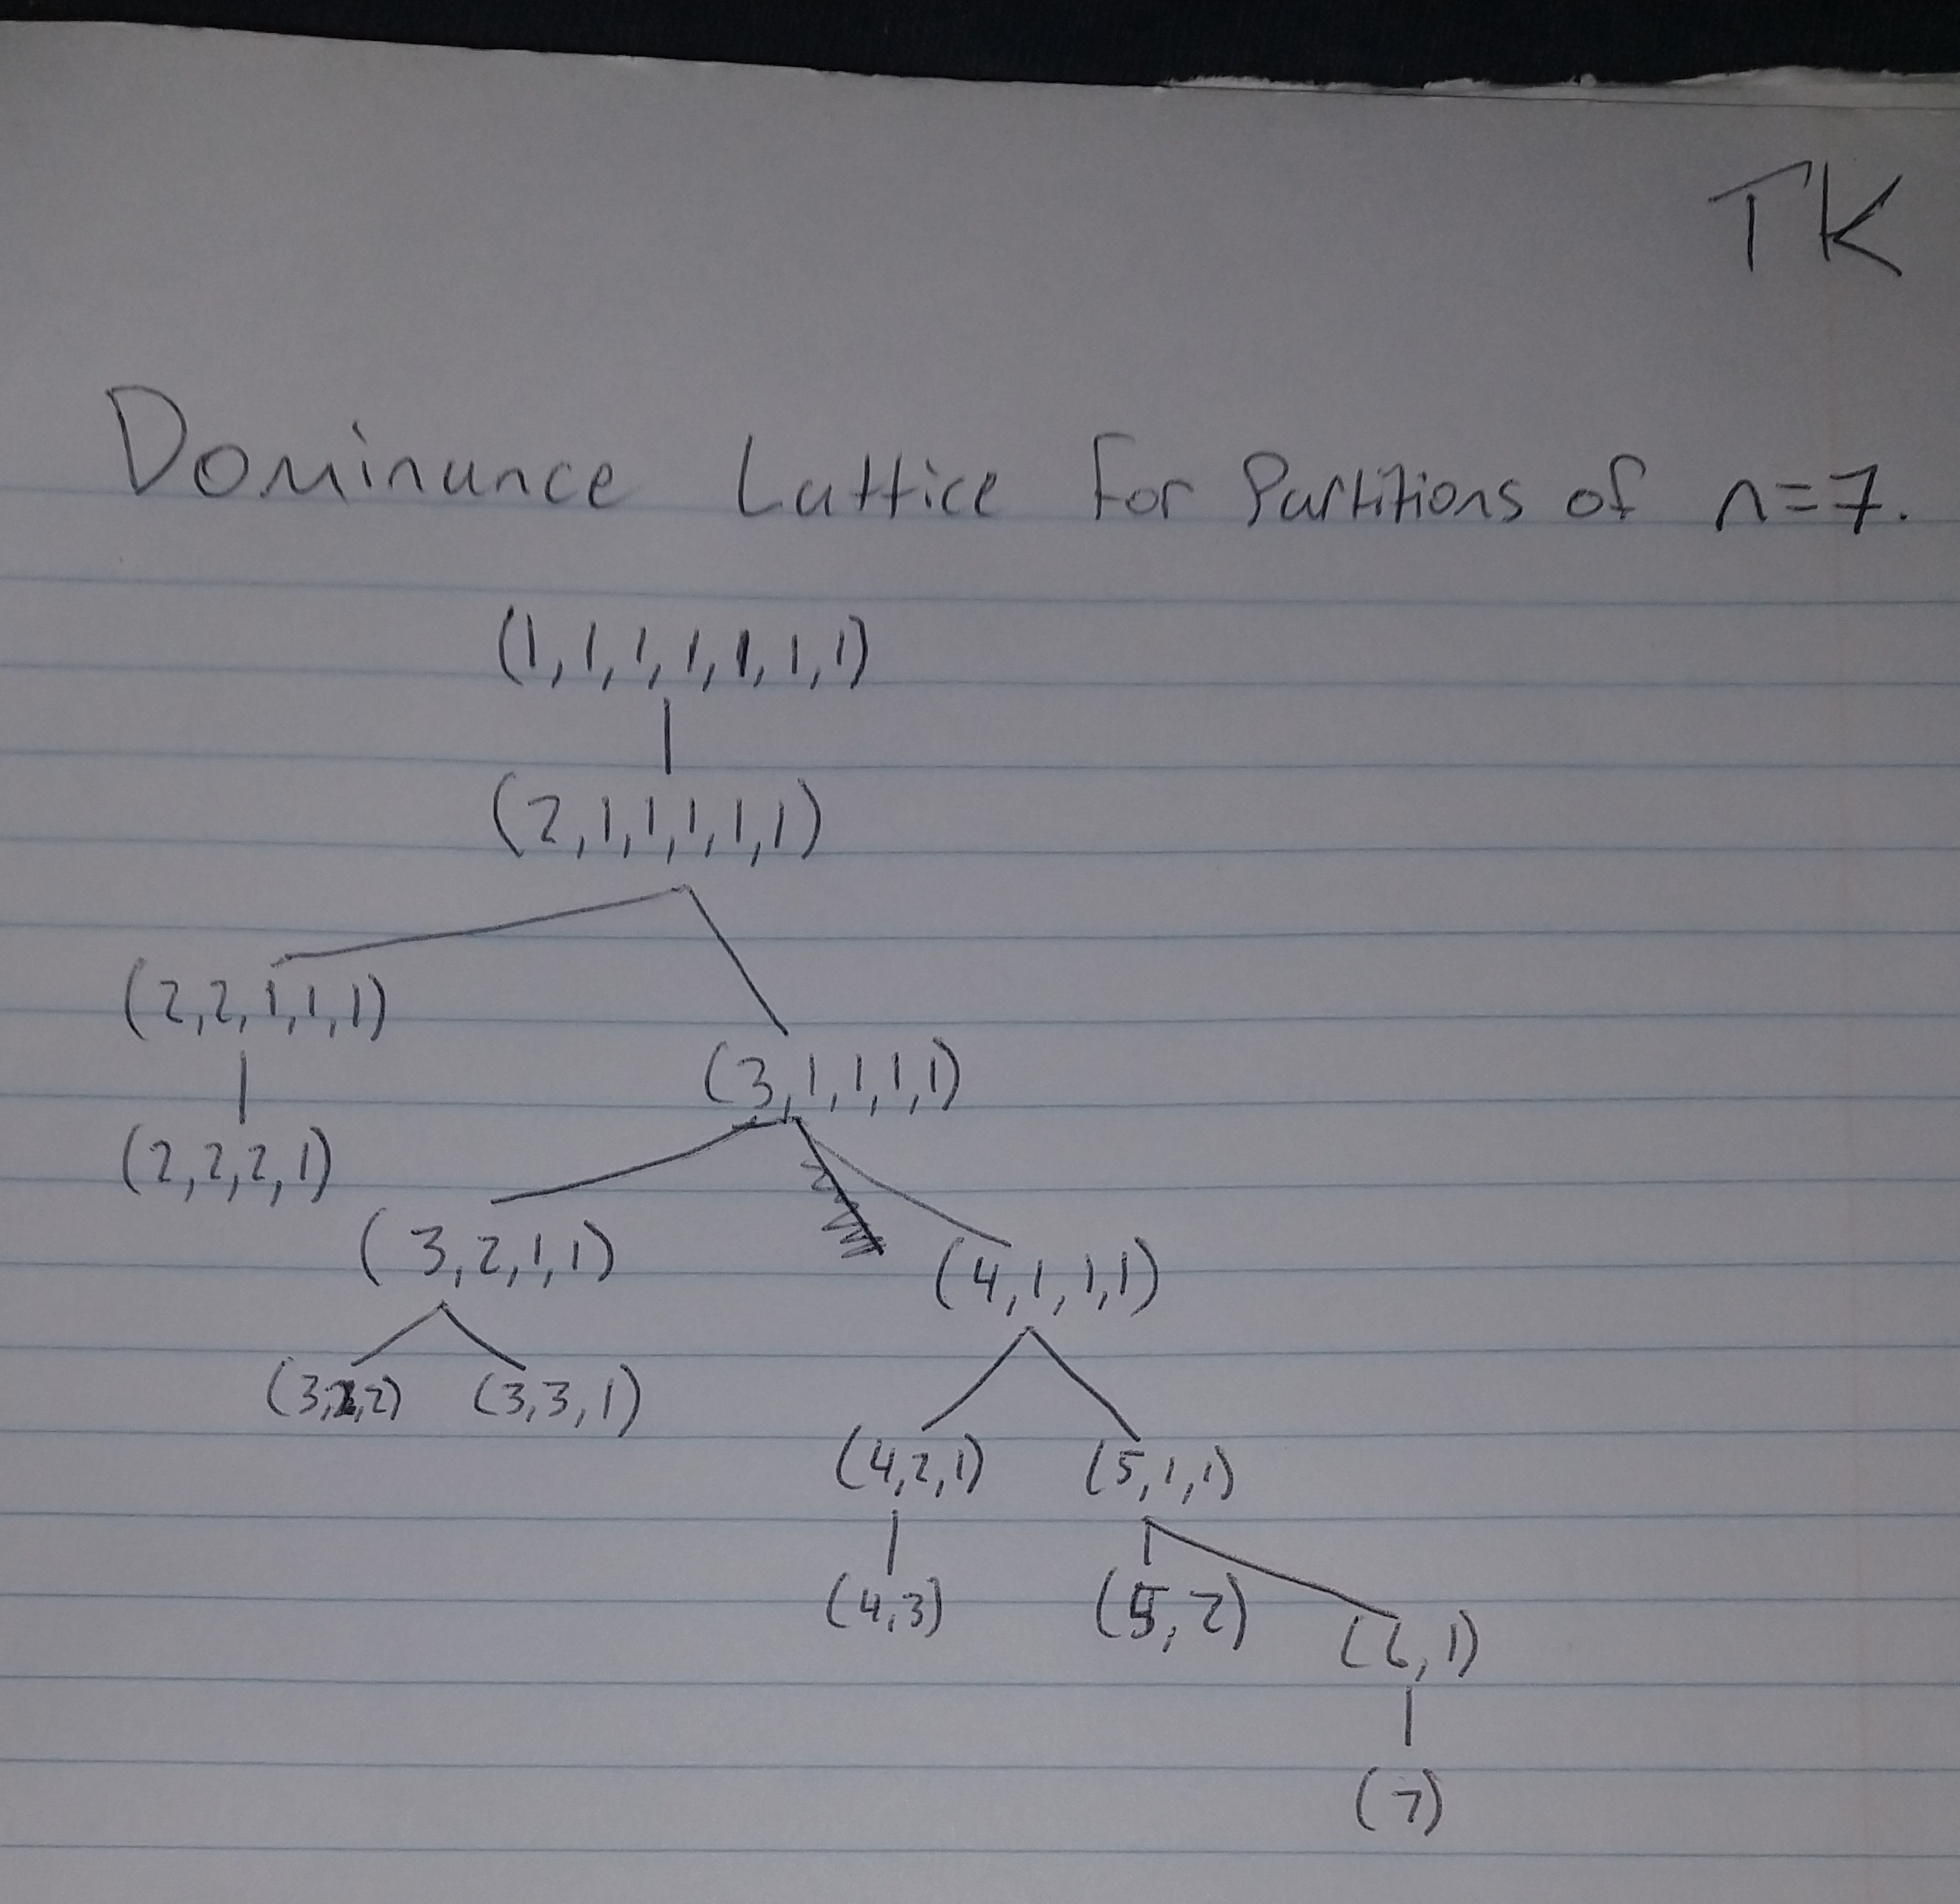
\includegraphics{DomLat}}
\end{enumerate}
\section{Circuit Problem:}
Convert the following to a Boolean Expression, then draw the corresponding simplified circuit.
\newpage\begin{enumerate}[label=(\alph*)]
    \item $a'\vee b'\vee(a\wedge b\wedge c')=a'\vee b'\vee c'$
    \newline\scalebox{.25}{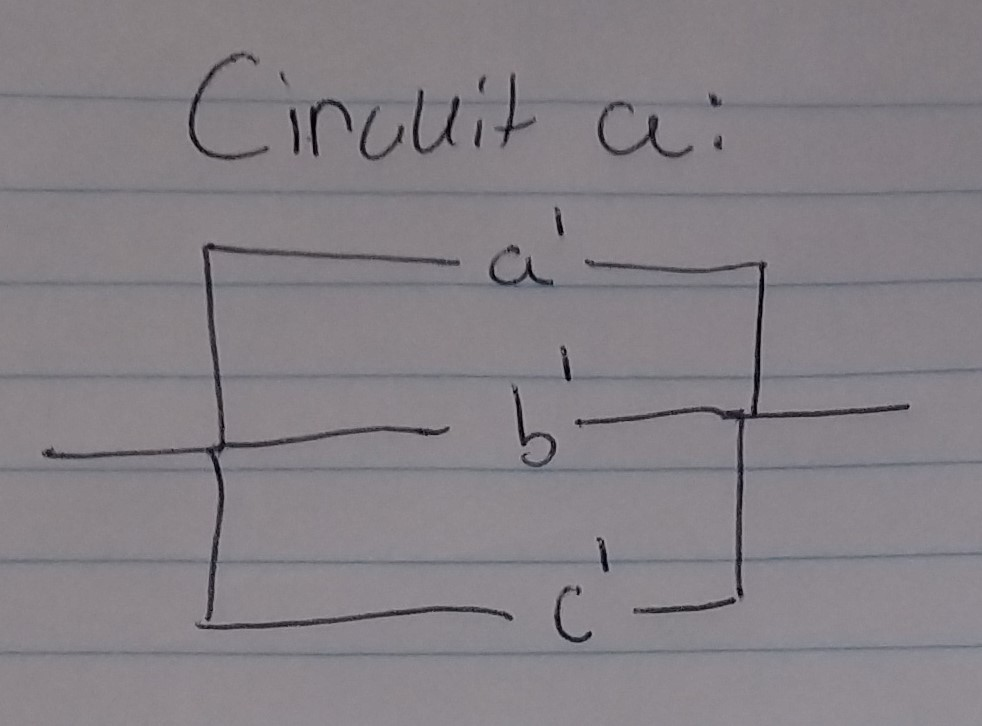
\includegraphics{FinalBool1}}
    \item $(a\wedge c)\vee(a'\wedge b)\vee(b\wedge c)=(a\wedge c)\vee(a'\wedge b)$
    \newline\scalebox{.2}{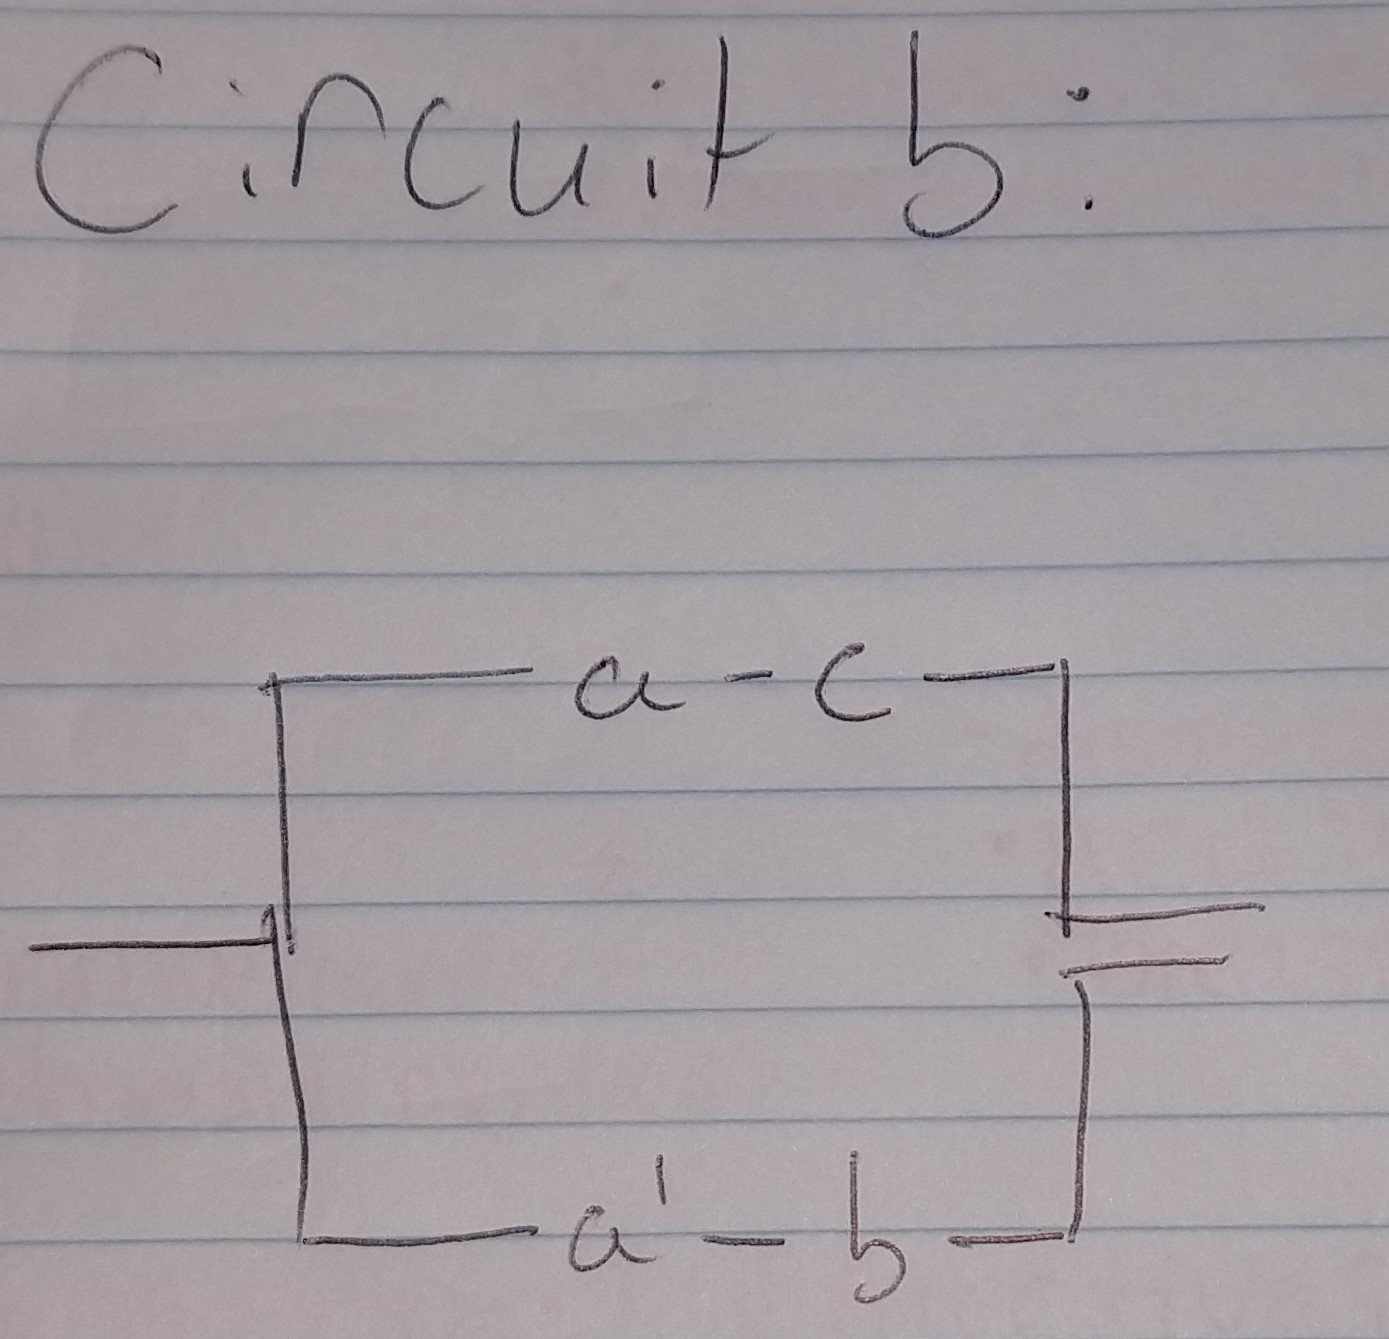
\includegraphics{FinalBool2}}
    \newpage\item $(a\vee c)\wedge(a'\vee b)\wedge(b\vee c)=(a\wedge b)\vee(a'\wedge c)$
    \newline\scalebox{.22}{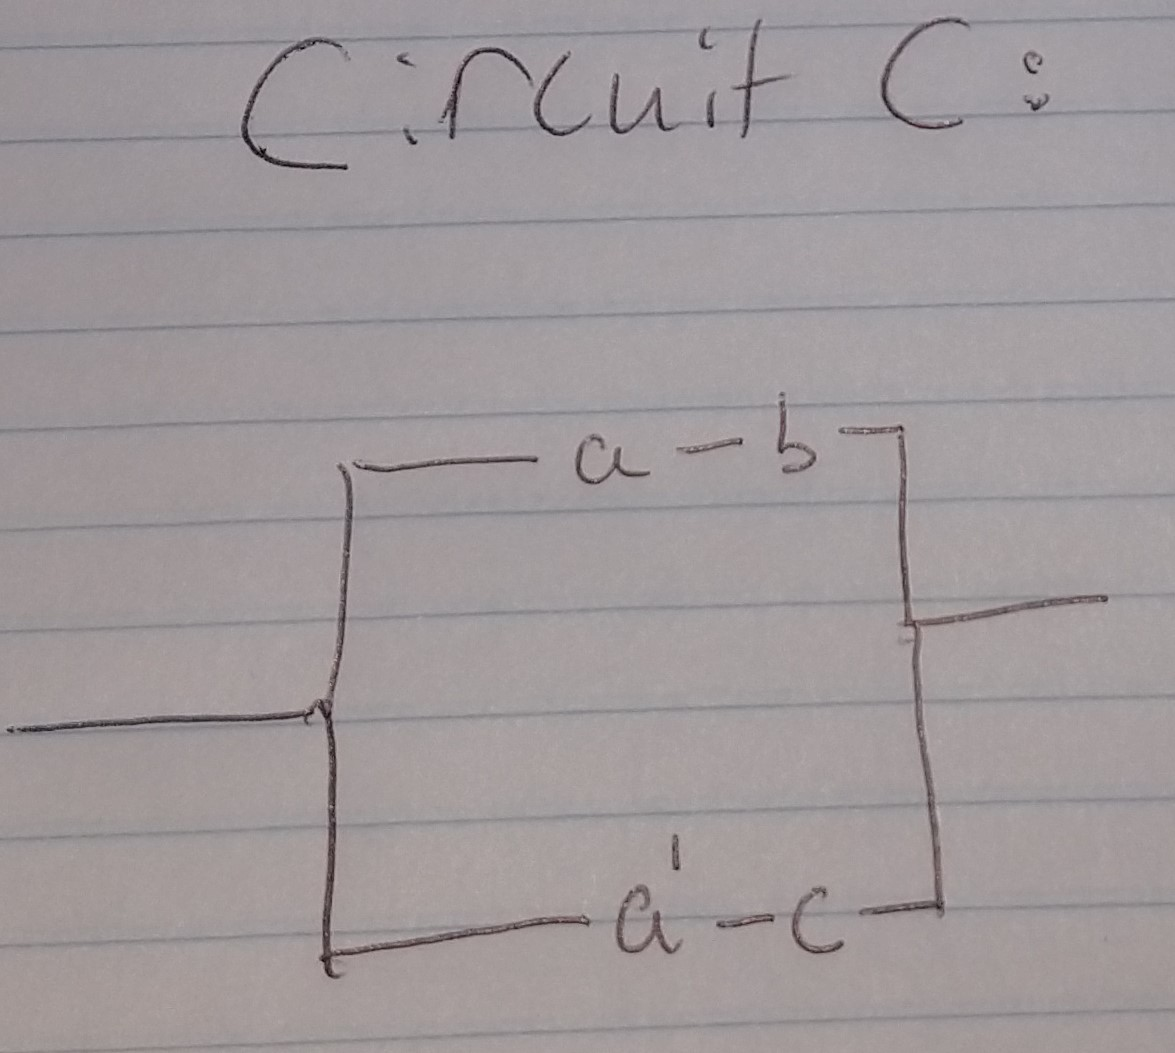
\includegraphics{FinalBool3}}
\end{enumerate}
\section{Boolean Algebra Problem:}
Simplify each of the following circuits using Boolean Algebra, and DeMorgan's Laws.
\begin{itemize}
    \item $((a\vee d)'\wedge(b'\vee c)')'=((a'\wedge d')\wedge(b\wedge c'))'=a\vee d\vee b'\vee c=a\vee b'\vee c \vee d$.
    \item $((a\wedge b \wedge c')'\vee(c'\wedge d)')'=a\wedge b\wedge c'\wedge d$.
    \item $(a'\vee d)'\wedge(b\vee c')'\wedge(c'\vee d)'=a\wedge b'\wedge c\wedge d'$.
\end{itemize}
\section{Necklace Problem:}
\begin{enumerate}[label=(\alph*)]
    \item Find all elements in the dihedral group $D_{14}$ of order fourteen. Write these  elements in cycle notation.
    \newline $D_{14}=\{r,r^2,r^3,r^4,r^5,r^6,r^7,s,sr,sr^2,sr^3,sr^4,sr^5,sr^6\}$
    \begin{enumerate}[label=(\roman*)]
        \item $r=(1234567)$
        \item $r^2=(1357246)$
        \item $r^3=(1473625)$
        \item $r^4=(1526374)$
        \item $r^5=(1642753)$
        \item $r^6=(1765432)$
        \item $r^7=(1)$
        \item $s=(1)(27)(36)(45)$
        \item $sr=(12)(37)(46)(5)$
        \item $sr^2=(13)(2)(47)(56)$
        \item $sr^3=(14)(23)(57)(6)$
        \item $sr^4=(15)(24)(3)(67)$
        \item $sr^5=(16)(25)(34)(7)$
        \item $sr^6=(17)(26)(35)(4)$
    \end{enumerate}
    \item Find the cycle index of $D_{14}$ acting on the regular hexagon.
$$f(x_1,x_2,x_3,x_4,x_5,x_6,x_7)=\frac{1}{14}\sum_{g\in D_{14}}=f_g$$
\begin{enumerate}[label=(\roman*)]
    \item $x_1^7=(1)(2)(3)(4)(5)(6)(7)$
    \item $x_7=(1234567)$
    \item $x_7=(1357246)$
    \item $x_7=(1473625)$
    \item $x_7=(1526374)$
    \item $x_7=(1526374)$
    \item $x_7=(1642753)$
    \item $x_1x_3^2=(1)(27)(36)(45)$
    \item $x_1x_3^2=(12)(37)(46)(5)$
    \item $x_1x_3^2=(13)(2)(47)(56)$
    \item $x_1x_3^2=(14)(23)(57)(6)$
    \item $x_1x_3^2=(15)(24)(3)(67)$
    \item $x_1x_3^2=(16)(25)(34)(7)$
    \item $x_1x_3^2=(17)(26)(35)(4)$
\end{enumerate}
So $$f(x_1,x_2,x_3,x_4,x_5,x_6,x_7)=\frac{1}{14}(x_1^7+6x_7+7x_1x_3^2)$$
    \item Find the pattern inventory of $D_{14}$ acting on $X$, the set of 7-bead necklaces in the colors W=White, B=Black, G=Gray. $$R=\{W,B,G\},f((W+B+G),(W^2+B^2+G^2),(W^3+B^3+G^3),...,(W^7+B^7+G^7))$$ $$=\frac{1}{14}[(W+B+G)^7+6(W^7+B^7+G^7)+7(W+B+G)(W^3+B^3+G^3)^2]$$
    \item The pattern inventory tells us exactly how many distinct necklaces with any number of white, black and gray beads are possible. You would calculate the total number of necklaces by plugging in 3 for all of $\{x_1,x_3,...,x_7\}$ and evaluating using the cycle index above.
\end{enumerate}
\section{Proof Problem (Group Actions):}
Suppose that $G$ is a group acting on a set $X$. For any element $x\in X$, prove that the set Stab$(x)$ is a subgroup of $G$.
\begin{proof}
The stabilizer of $x\in G$, Stab$(x)$ is defined as the elements $g$ in $G$ that fix $x$, that is:$$\text{Stab}(x)=\{g\in G|g\cdot x=x\}$$ N2S: \begin{enumerate}
    \item $e\in\text{Stab}(x)$
    \item $\forall a\in\text{Stab}(x),a^{-1}\in\text{Stab}(x)$
    \item $\forall a,b\in\text{Stab}(x),a\cdot b\in\text{Stab}(x)$
\end{enumerate}(no need to show commutativity because it is inherited from $G$).\newline (1).\newline Of course, the identity element $e\in\text{Stab}(x)$, because it doesn't change anything and therefore fixes $x$.\newline(2).\newline Consider the element $a\in\text{Stab}(x)$. Thus, by definition of $\text{Stab}(x)$, $a(x)=x$. Since $x=a(x)$, $x=a^{-1}(a(x))=a^{-1}(x)$, therefore, since $a^{-1}$ fixes $x$, $a^{-1}\in\text{Stab}(x)$.\newline(3).\newline Finally, consider two elements $a,b\in\text{Stab}(x)$, again, $a(x)=x$ and $b(x)=x$. $ab(x)=a(b(x))=a(x)=x$, and $ba(x)=b(a(x))=b(x)=x$. So $\forall a,b\in\text{Stab}(x),a\cdot b\in\text{Stab}(x)$. As required, therefore $\text{Stab}(x)\leq G$.
\end{proof}
\end{document}